\documentclass{article}
\usepackage{amsmath}
\usepackage{graphicx}
\usepackage[T1]{fontenc}
\graphicspath{{images/}}
\title{List 3 report}
\author{Albert Kołodziejski}
\begin{document}
\maketitle

\section*{Exercise 1}

\subsection*{Description of problem:}
This exercise requires to implementation of the bisection method, which is used to find the root of a given function.

\subsection*{Description of method:}
Suppose we want to compute the root of function f, if we have some range [a,b] such that f(a)f(b) < 0, that would mean zero point is between a and b, therefore we can try to make this range smaller and smaller while also narrowing down possible values of the root. The bisection method takes a middle of a range (c), check in which half function changes sign, [a, c] or [c, b]. For the chosen new range it again tries to narrow down zero point. 

\begin{center}
    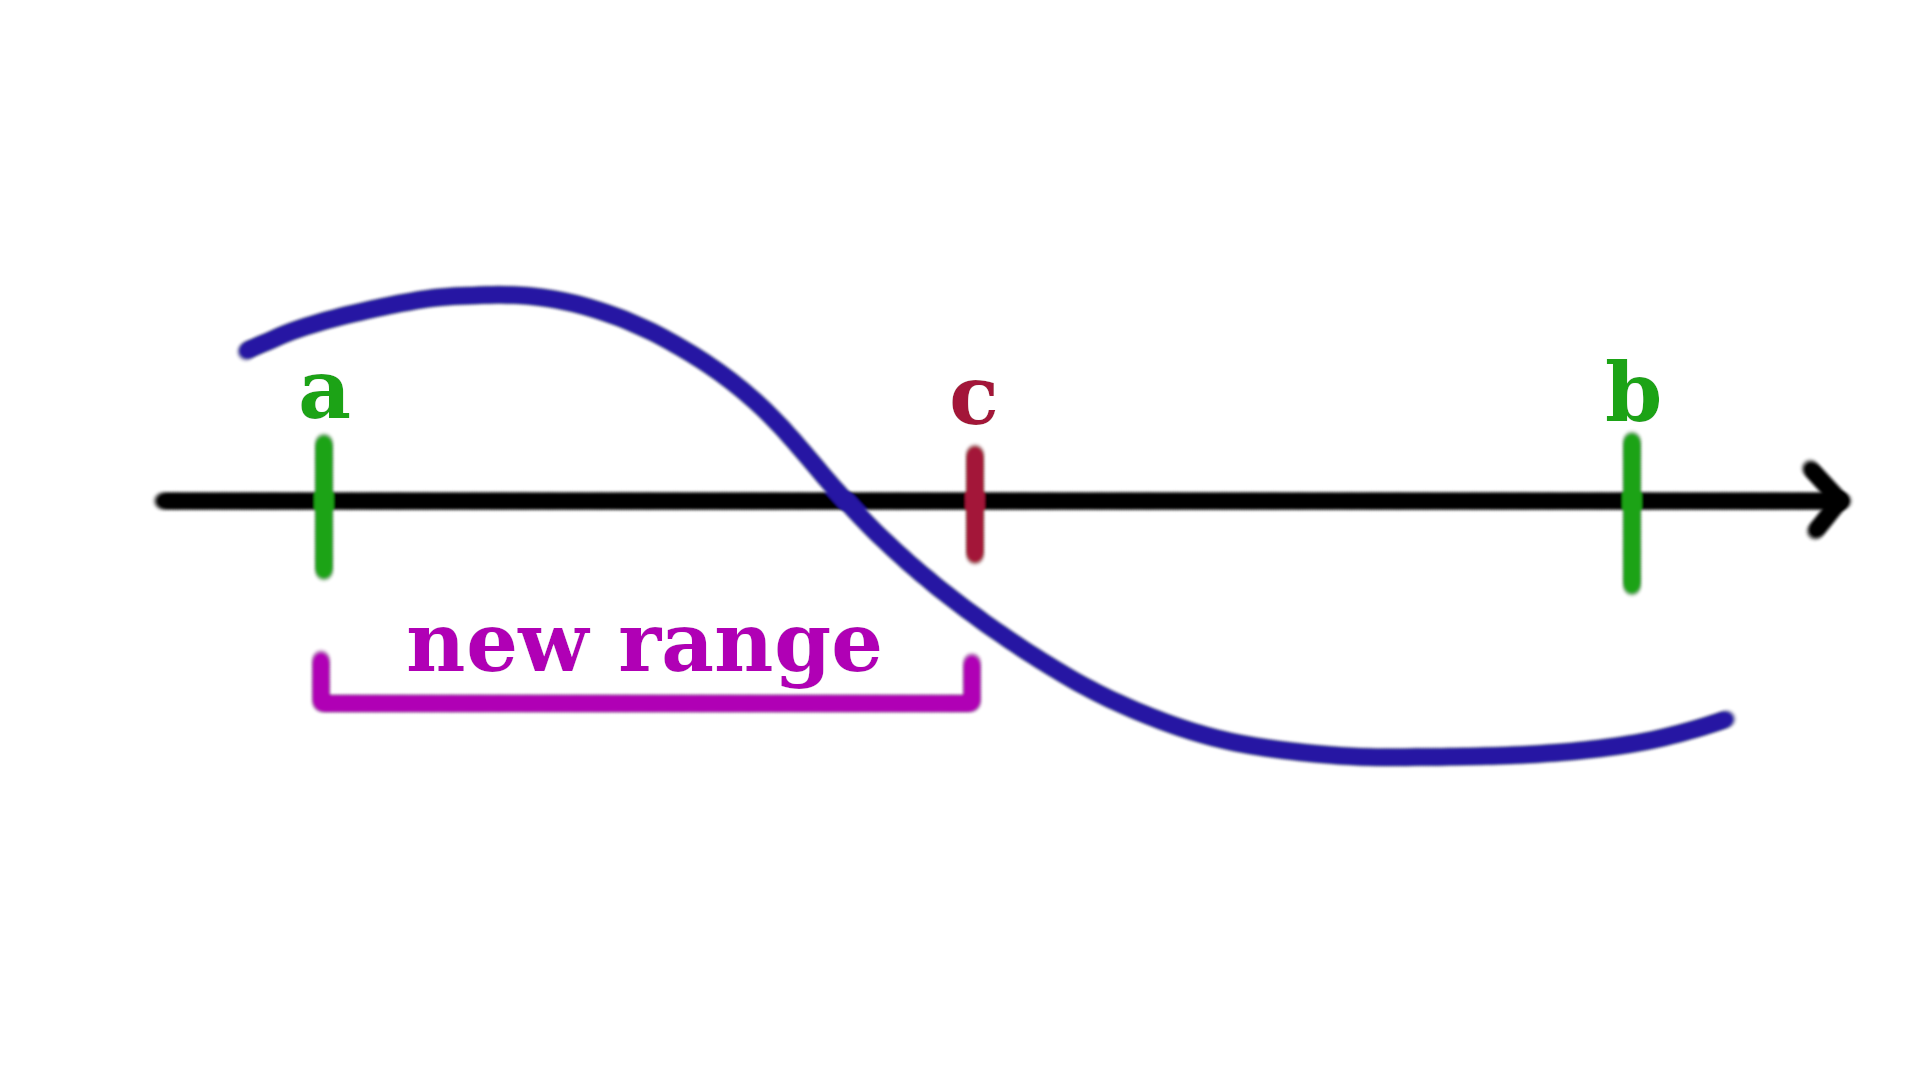
\includegraphics[scale=0.7]{bisection}
\end{center}

We do it until the length of the range is smaller than a given delta, or |f(c)| is smaller than a given epsilon.

\section*{Exercise 2}

\subsection*{Description of problem:}
This exercise requires to implementation of Newton's method, which is used to find the root of a given function.

\subsection*{Description of method:}
Suppose we want to compute the zero point of function f and we know its derivative. 


\begin{center}
    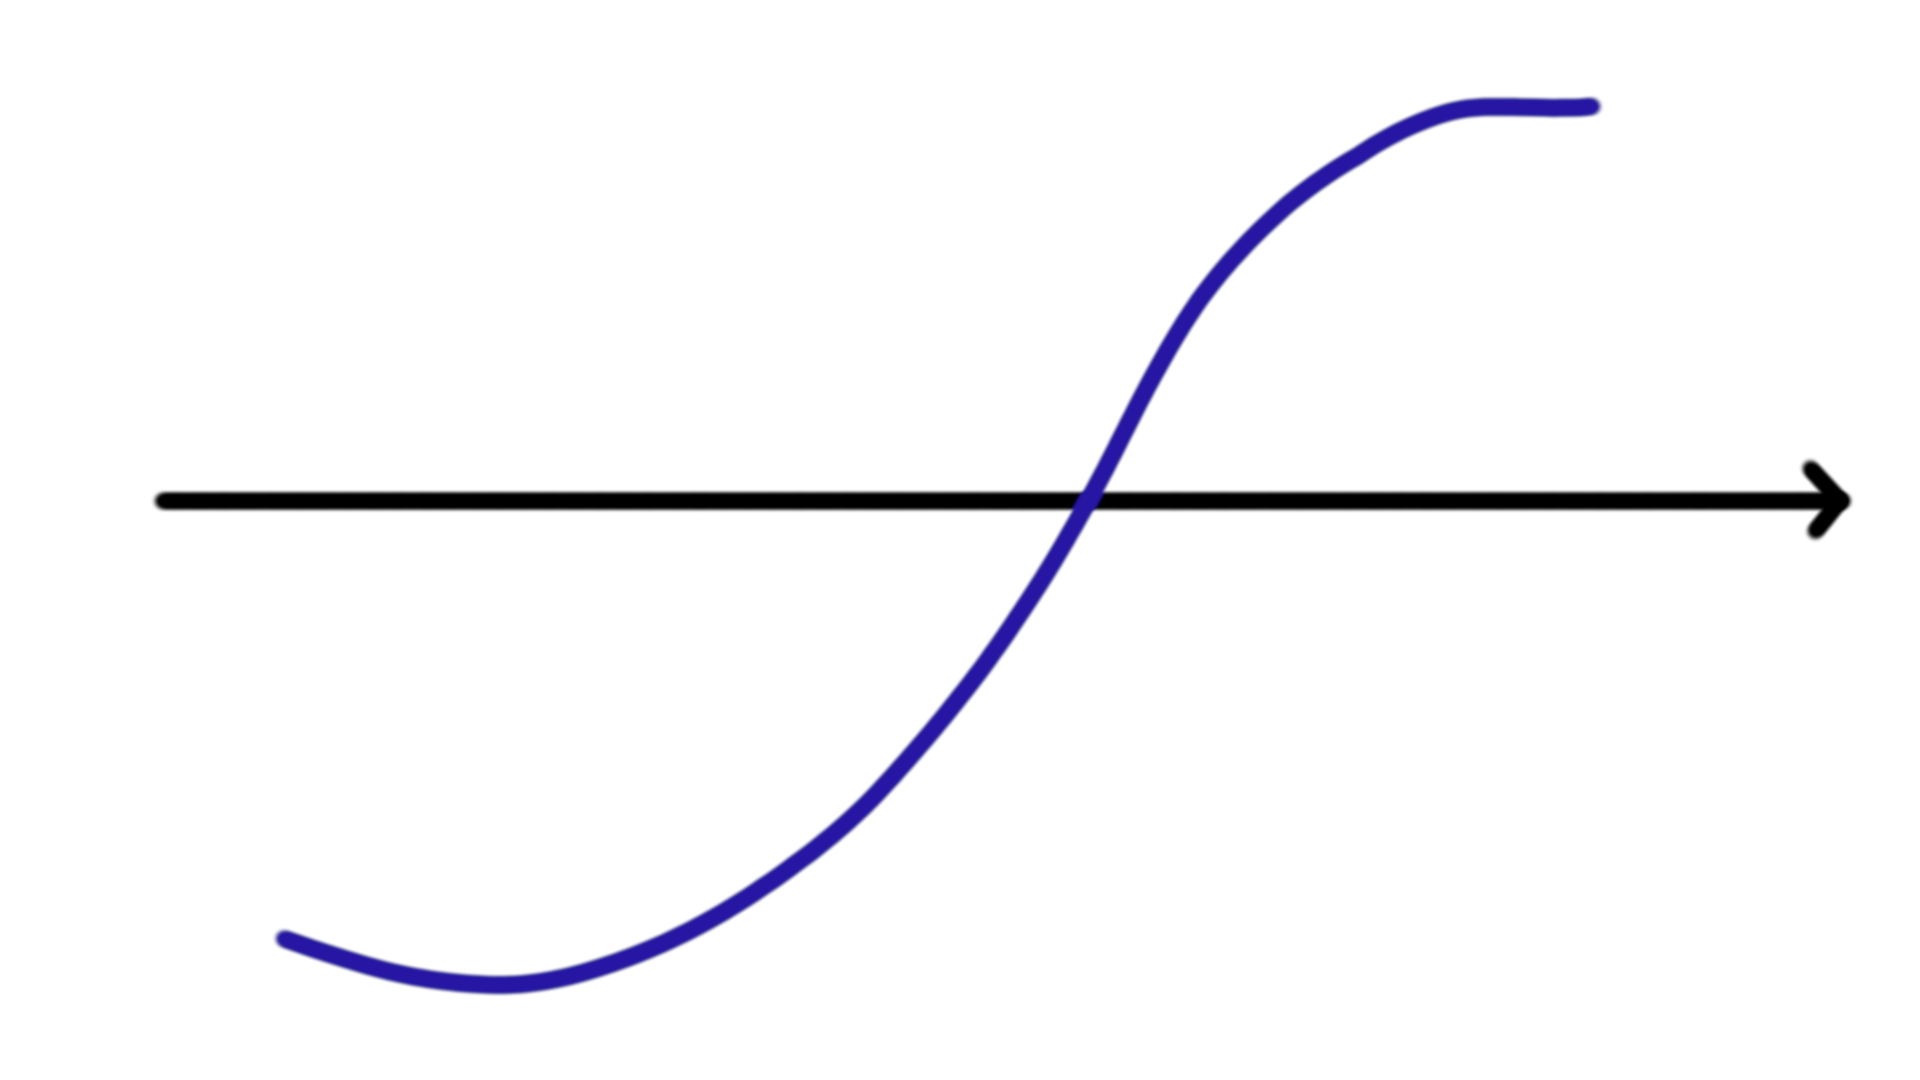
\includegraphics[scale=0.3]{newton1}
\end{center}
We can take some point on the x-axis, and from the derivative, we can get a rate of change at that point, and if the function doesn't drastically change the rate of change between our point and zero point, the point of intersection of the tangent with the x-axis should get as closer to zero point.

\begin{center}
    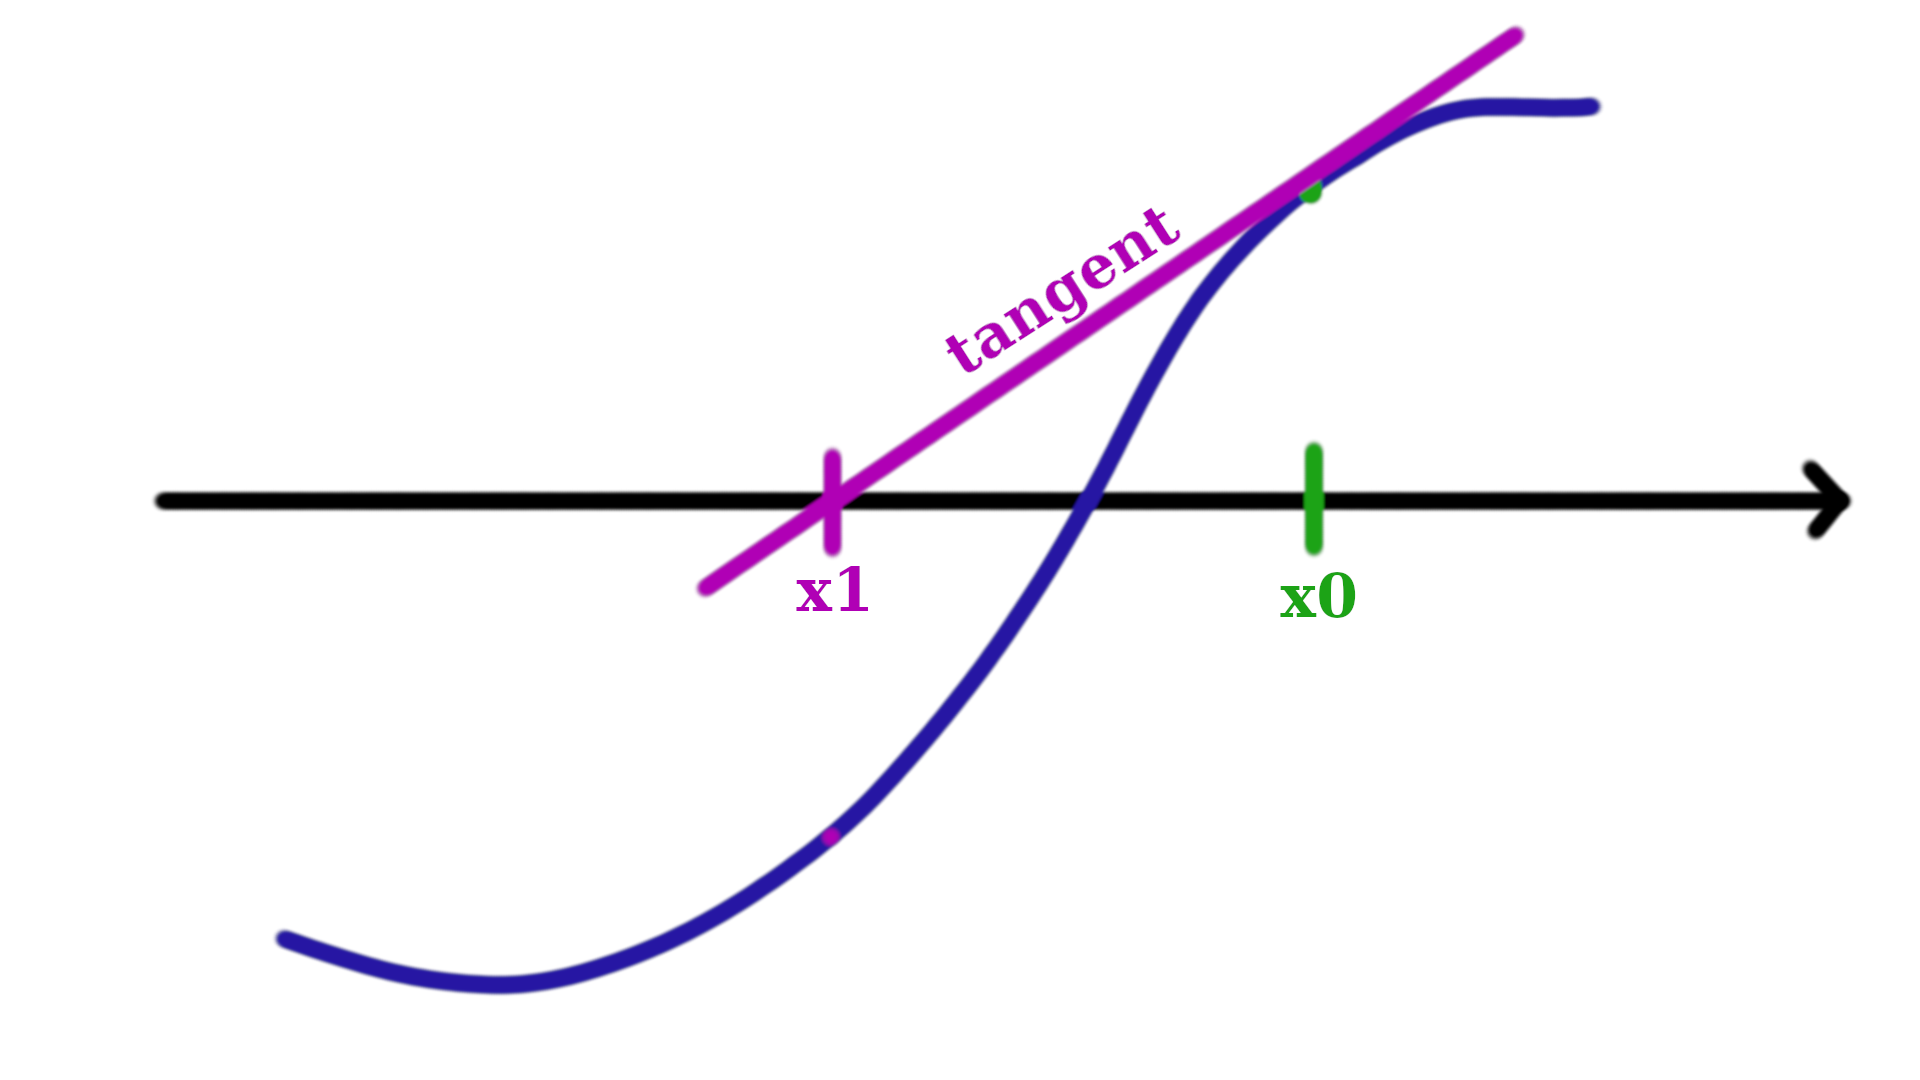
\includegraphics[scale=0.3]{newton2}
\end{center}
Now point of intersection is our new point, for which we do the same thing.

\begin{center}
    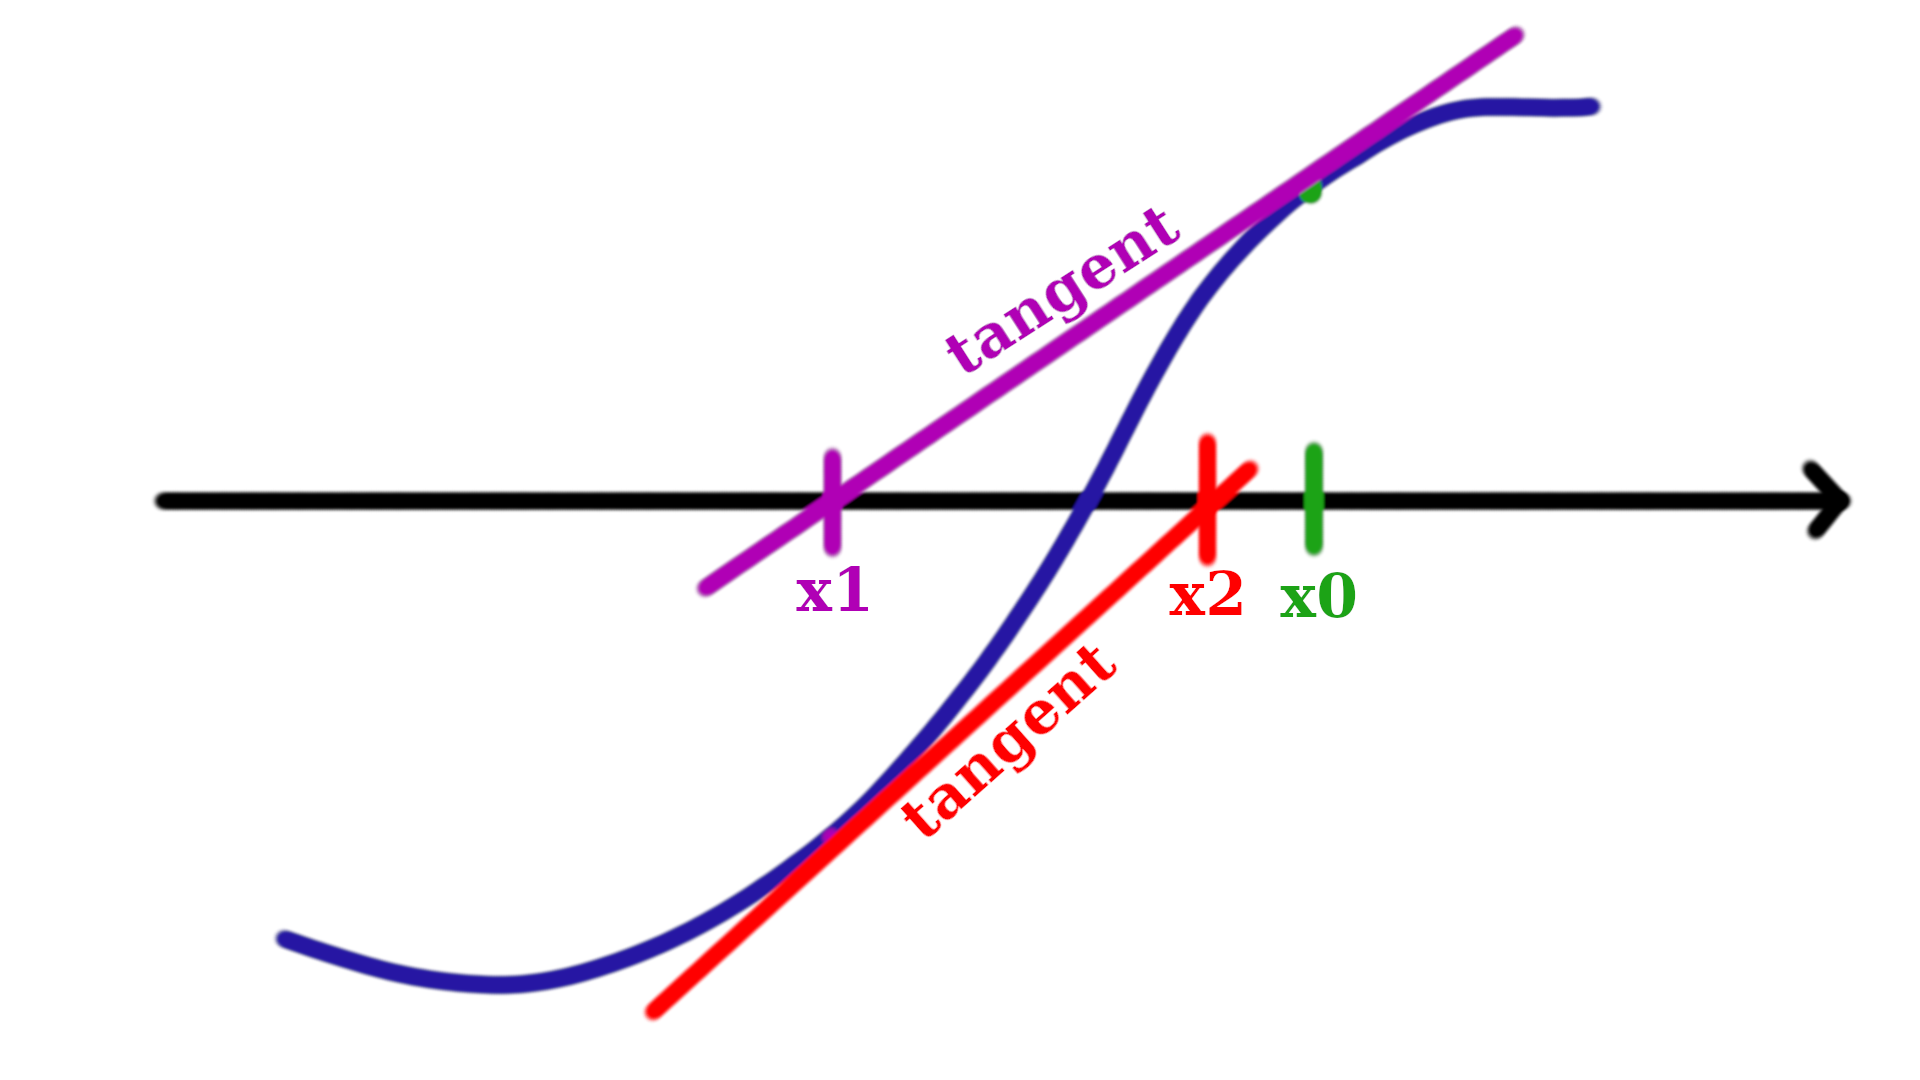
\includegraphics[scale=0.4]{newton3}
\end{center}

Newton's method is those steps repeated some amount of times until the distance between x\textsubscript{n} and x\textsubscript{n + 1} is smaller than a given delta or |f(x\textsubscript{n + 1})| is smaller than a given epsilon. It is important to give a restriction on the number of times a function can iterate because it sometimes cannot converge to any value.

\section*{Exercise 3}
\subsection*{Description of problem:}
This exercise requires to implementation of the secant method, which is used to find a root of a given function.

\subsection*{Description of method:}
Suppose we want to compute a root of function f.

\begin{center}
    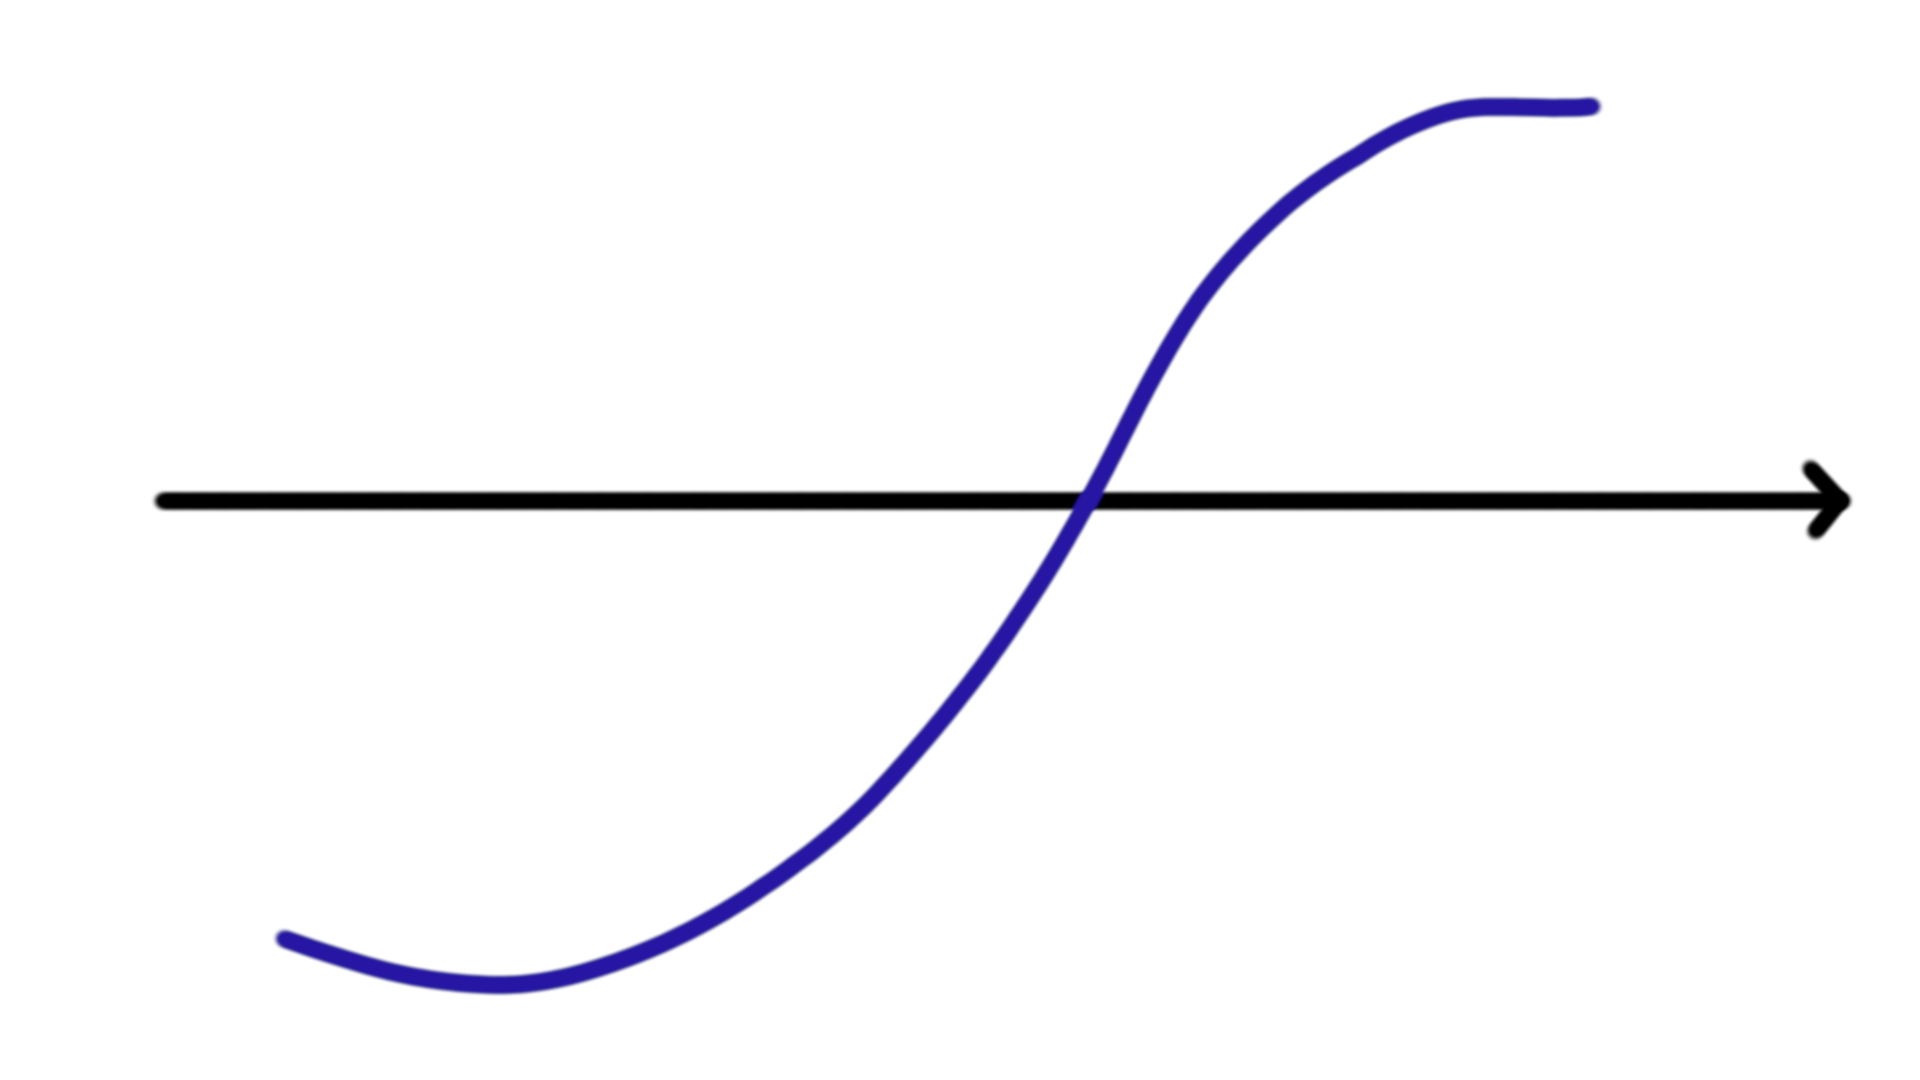
\includegraphics[scale=0.3]{newton1}
\end{center}

We can take some 2 points, and connect them through the line, which can be interpreted as an approximation of function, with the difference that computing the root for it is much simpler. If our function doesn't drastically change between our points and the root that we are looking for, the point of intersection of approximation should get closer to the root.

\begin{center}
    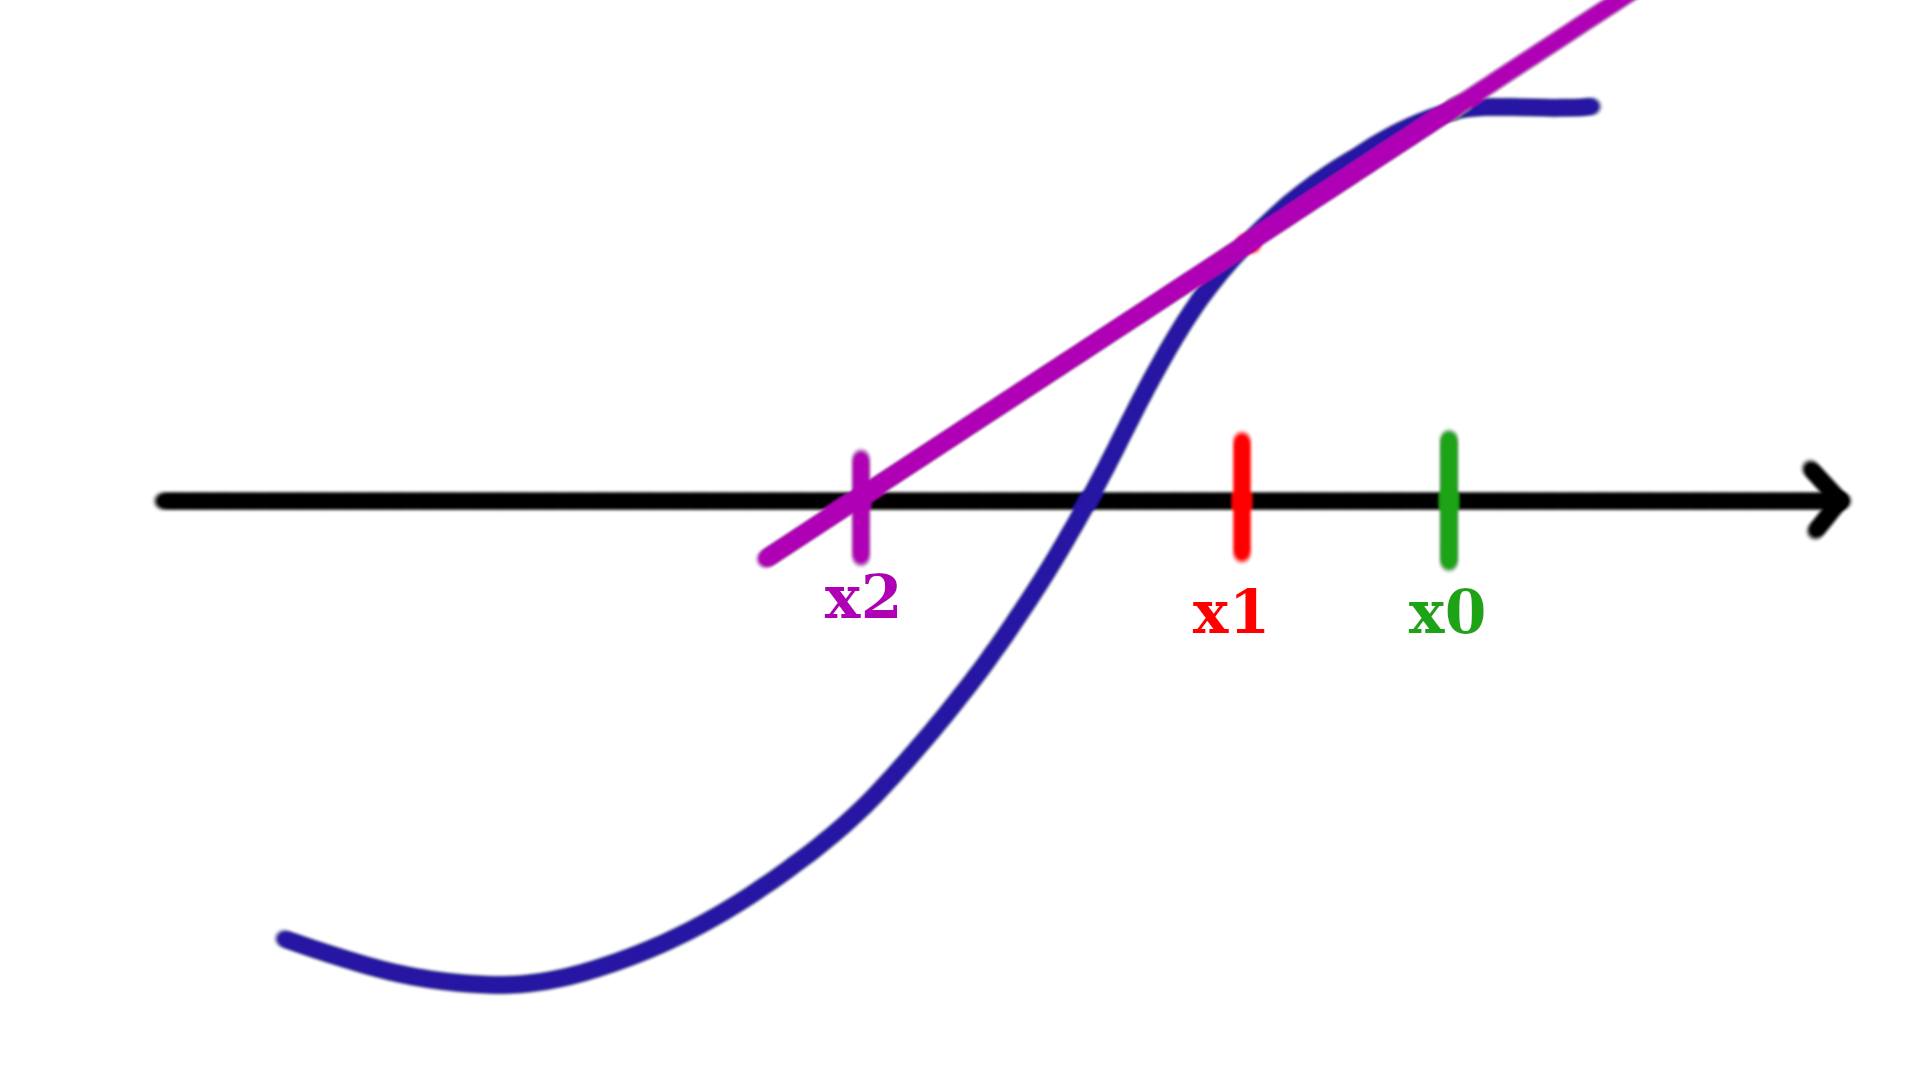
\includegraphics[scale=0.3]{secant1}
\end{center}
Now we can do the same for one of our previous points, and point of intersection.

\begin{center}
    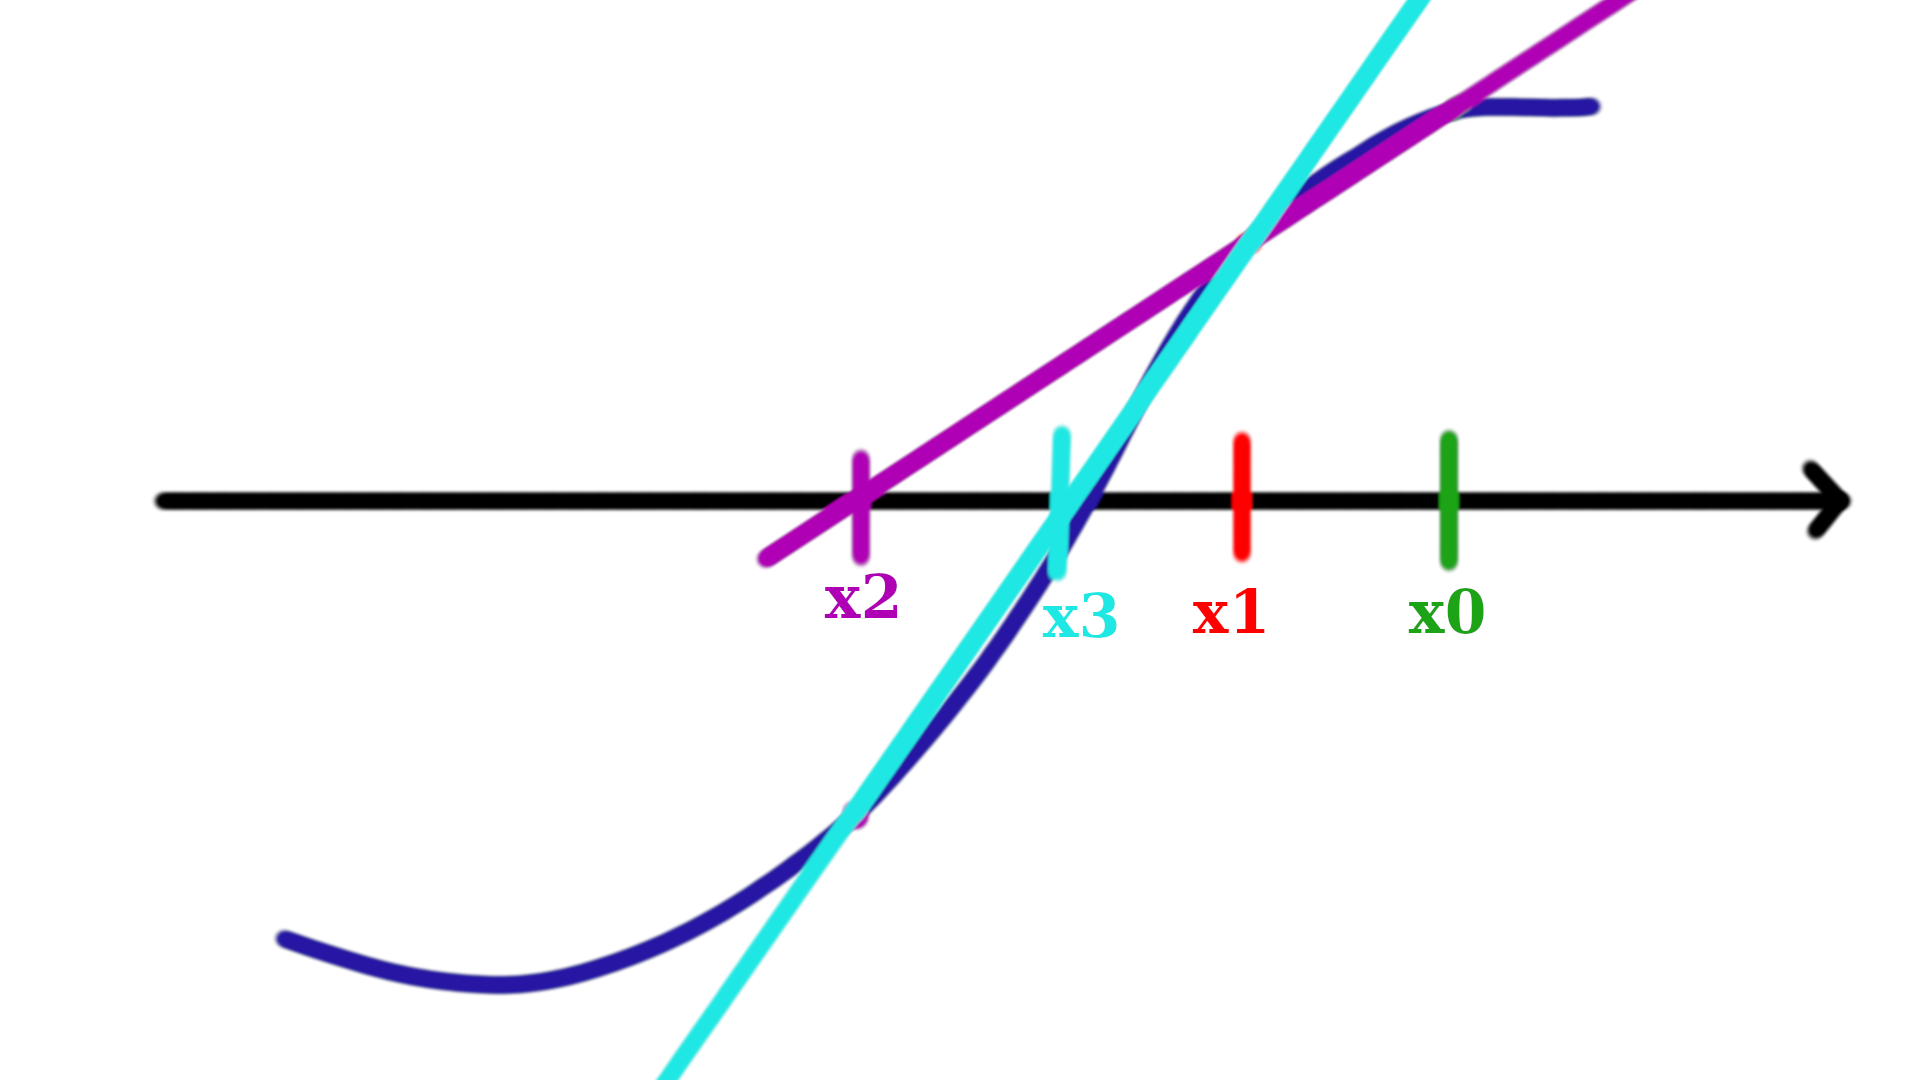
\includegraphics[scale=0.3]{secant2}
\end{center}

The Secant method is exactly that, repeated some amount of times until the distance between x\textsubscript{n} and x\textsubscript{n + 1} is smaller than given delta or |f(x\textsubscript{n + 1})| is smaller than given epsilon. It is important to give a restriction on the number of times a function can iterate because it sometimes cannot converge to any value.


\section*{Exercise 4}
\subsection*{Description of problem:}
In this exercise we are going to numerically find the root of:

\[
    sin(x) - (\frac{1}{2}x)^2 = 0
\]

\subsection*{Results:}
\begin{center}
    \begin{tabular}{| c | c | c | c |}
        \hline
         method & x & f(x) & iterations \\ 
        \hline
        \hline
        Bisection & 1.9337539672851562 & -2.7027680138402843e-7 &  16 \\
        \hline
        Newton & 1.933753779789742 & -2.2423316314856834e-8 & 4 \\
        \hline
        Secant & 1.933753644474301 &  1.564525129449379e-7 & 4 \\
        \hline
    \end{tabular}
\end{center}

\subsection*{Interpretation and conclusions:}
The bisection method is the slowest when it comes to the number of iterations.

\section*{Exercise 5}
\subsection*{Description of problem:}
In this exercise we are going to use the bisection method to find the intersection of given functions:

\[
    y = 3x
\]
\[
    y = e^x
\]

\subsection*{Results:}
To do so we could find the roots of:

\[
    e^x - 3x = 0
\]

But firstly we need to know what ranges we need to work on, as the bisection method can only work when there is only one root in a given range. Here are a couple of facts that I came up with that will help us to make those ranges.

1) e\textsubscript{x} > 3x is true for every negative value because the left side will always be positive while the right is negative for negative x.

2) as e\textsubscript{x} grows faster than 3x, so from some point onward e\textsubscript{x} > 3x is always true

3) This function will have some minimum, to the left it will grow to infinity because of 1) and because 3x decreases faster to the left than e\textsubscript{x}, and to the right, it will grow to infinity because of 2), Final shape would look like some parabola, and as a parabola it will have, zero, one or two roots.

4) for x = 0:
\[
    e^x = e^0 = 1 > 0 = 3*0 = 3*x
\]

5) for x = 1:
\[
    e^x = e^1 \approx 2.7 < 3 = 3*1 = 3*x
\]

6) for x = 2:
\[
    e^x = e^2 \approx 7 > 6 = 3*2 = 3*x
\]

That's why we know one root is in [0, 1], and second is in [1, 2]

\subsection*{Results:}
\begin{center}
    \begin{tabular}{| c | c | c | c |}
        \hline
        range & x & f(x) & iterations \\ 
        \hline
        \hline
        [0, 1] & 0.619140625 & -9.066320343276146e-5 & 9\\
        \hline
        [1, 2] & 1.5120849609375 & -7.618578602741621e-5 & 13\\
        \hline
    \end{tabular}
\end{center}

\subsection*{Interpretation and conclusions:}
Those methods can not find all roots on their own, they need to be prepared with correct operands.

\section*{Exercise 6:}
\subsection*{Description of the problem:}
In this exercise we are going to use all methods to compute the roots of two functions:
\[
    f_1(x)  = e^{1-x} -1
\]
\[
    f_2(x)  = xe^{-x}
\]

\subsection*{Results:}
After some trial and error, I came up with those results:
\\
\\
For f\textsubscript{1} there is one root equal to 1:
\begin{center}
    \begin{tabular}{| c | c | c | c |}
        \hline
         method & x & f\textsubscript{1}(x) & iterations \\ 
        \hline
        \hline
        Bisection, [-3.14, 1.618] & 0.99999942779541 & 5.722047538014863e-7 & 18 \\
        \hline
        Newton, x\textsubscript{0} = -1.0& 0.9999922654776594 & 7.734552252003368e-6 & 5\\
        \hline
        Secant, x\textsubscript{0} = -1.0, x\textsubscript{1} = -2.0 & 0.999999927401123 & 7.259887957467015e-8 & 8 \\
        \hline
    \end{tabular}
\end{center}
\newpage
For f\textsubscript{2} there is one root equal to 0:
\begin{center}
    \begin{tabular}{| c | c | c | c |}
        \hline
         method & x & f\textsubscript{2}(x) & iterations \\ 
        \hline
        \hline
        Bisection, [-3.14, 1.618] & 7.019042968630344e-6 & 7.018993701839051e-6 & 15 \\
        \hline
        Newton, x\textsubscript{0} = -1.0& -3.0642493416461764e-7 & -3.0642502806087233e-7 & 5\\
        \hline
        Secant, x\textsubscript{0} = -1.0, x\textsubscript{1} = -2.0 & -6.982568902521766e-6 & -6.982617658960467e-6 & 7 \\
        \hline
    \end{tabular}
\end{center}
\subsection*{QA:}
\begin{center}
    \textbf{What happens when for the first function we try Newton method with \textit{\(x_0 \in (1, \infty)\)}?}
\end{center}
\begin{center}
    \begin{tabular}{| c | c | c |}
        \hline
         x\textsubscript{0} & result & iterations \\ 
        \hline
        \hline
        2 & 0.9999999810061002 & 5 \\
        \hline
        3 & 0.9999999710783241 & 9 \\
        \hline
        4 & 0.9999999995278234 & 21 \\
        \hline
        5 & 0.9999996427095682 & 54 \\
        \hline
        6 & 0.9999999573590406 & 147 \\
        \hline
        7 & 0.9999999484165362 & 401 \\
        \hline
        8 & error: derivative too close to zero & 2 \\
        \hline
    \end{tabular}
\end{center}
As we can see the farther we go into this range, the more iterations it takes to find the root, and after 7 derivative is just too close to zero.
\begin{center}
    \textbf{What happens when for the second function we try Newton method with \textit{\(x_0 > 1\)}?}
\end{center}
For any starting value bigger than 1 we find a cheated root, that is not a real root, but it just happens that it is epsilon close to the x-axis.
\begin{center}
    \begin{tabular}{| c | c | c |}
        \hline
         x\textsubscript{0} & result & iterations \\ 
        \hline
        \hline
        1.1 & 14.272123938290509 & 3 \\
        \hline
        1.01 & 102.00999999999992 & 1 \\
        \hline
        1.001 & 1002.0010000001103 & 1 \\
        \hline
    \end{tabular}
\end{center}
Because this function slopes down after 1:

\begin{center}
    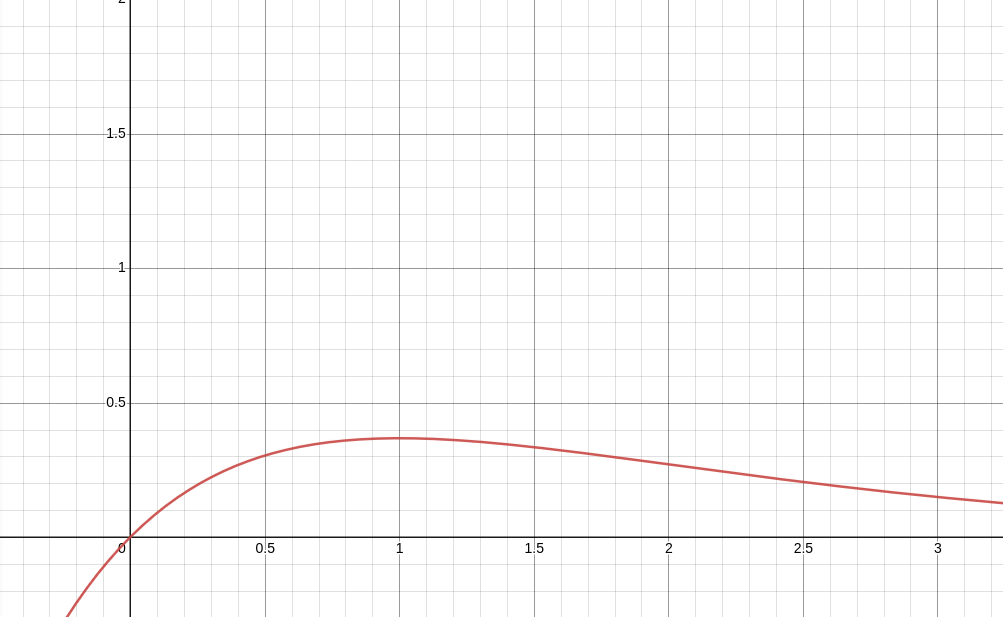
\includegraphics[scale=0.2]{first_function}
\end{center}

\begin{center}
    \textbf{What happens when for the second function we try Newton method with \textit{\(x_0 = 1\)}?}
\end{center}
For this point, Newton's method stops because the derivative is equal to zero.
\[
    f_2'(x) = -e^{-x}(x - 1) = -e^{-1}(1 - 1) = -e^{-1}0 = 0
\]

\end{document}